\documentclass[14pt]{extarticle}
\usepackage[export]{adjustbox}
\usepackage{multicol}
\usepackage[ocgcolorlinks]{hyperref}
\usepackage{graphicx}
\usepackage{geometry}
\geometry{tmargin=1em,bmargin=2em,
lmargin=2em,rmargin=2em}

\setlength\parindent{0pt}
\setlength{\columnsep}{1em}

\pagestyle{empty}

\begin{document}

\begin{center}

\includegraphics[width=0.3\textwidth]{H_SEAS_logo_RGB.jpg}
\\
\huge{PL/HCI Seminar (252R/279R)}\\
\large{MW 12-1:15 PM in LISE 303}\\
\end{center}

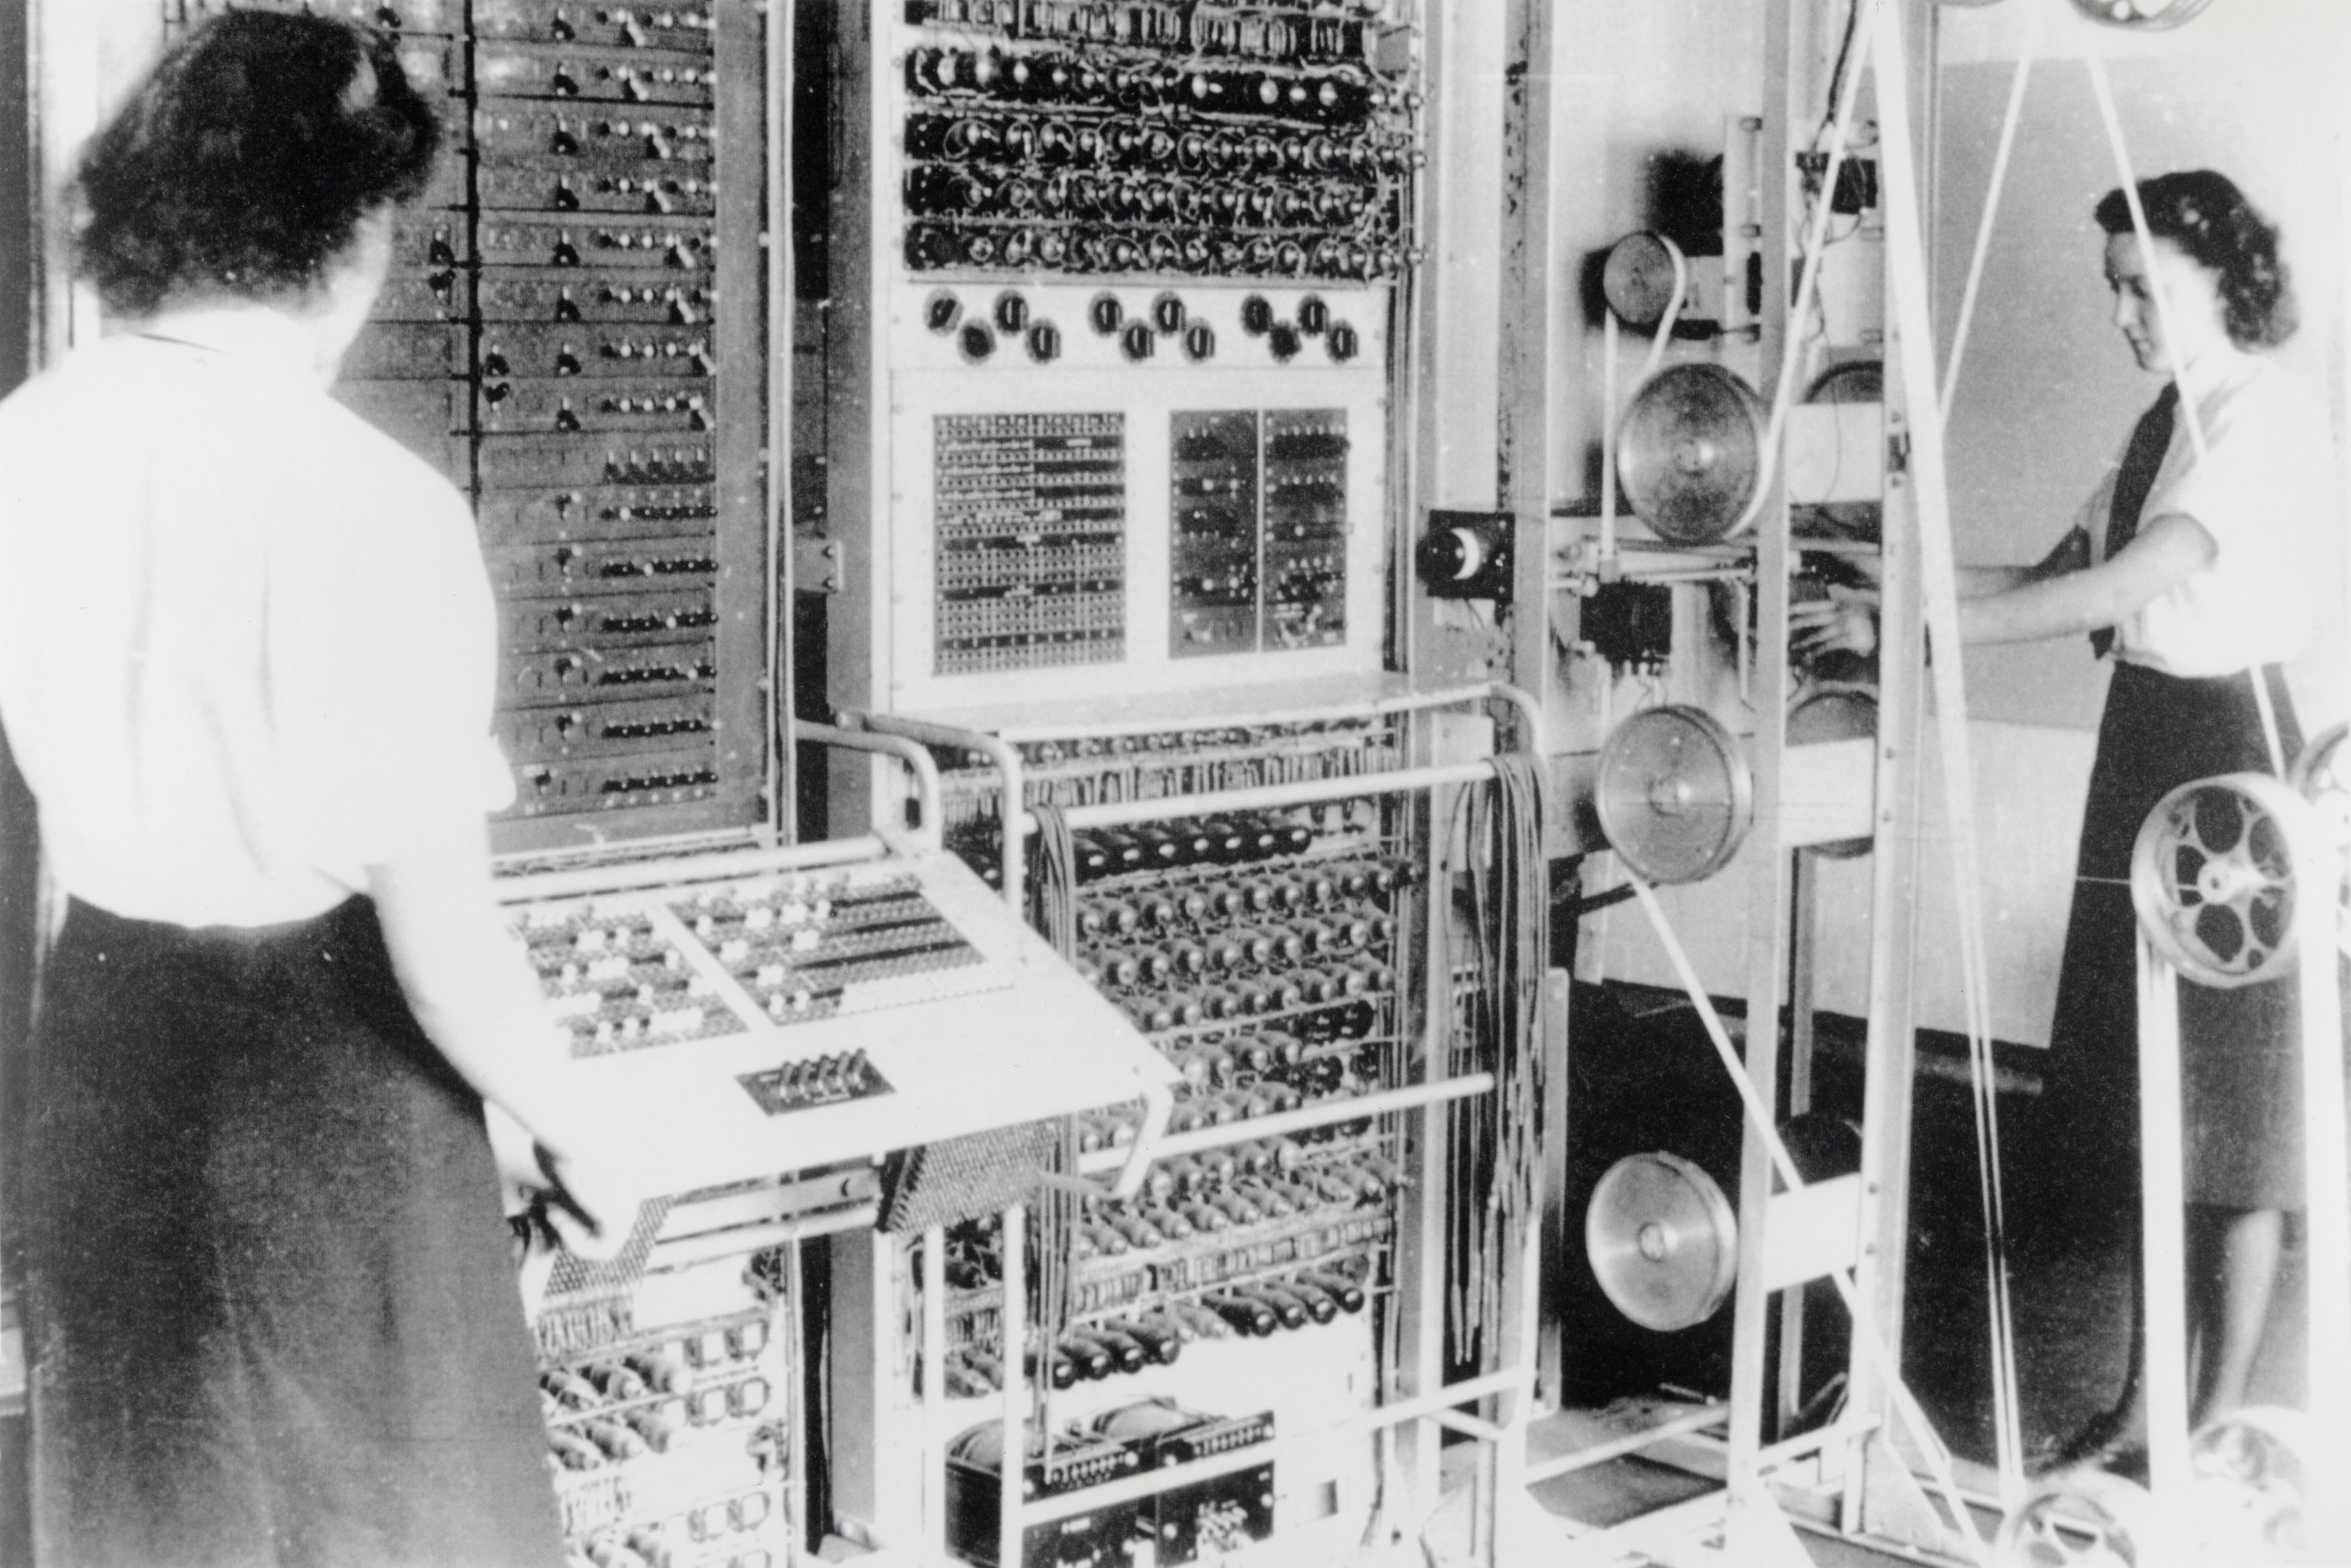
\includegraphics[width=\textwidth]{Colossus.jpg}




\begin{multicols}{2}
Programming Languages includes:
\begin{itemize}
\item Types
\item Synthesis
\item Metaprogramming
\end{itemize}

\columnbreak
Human-Computer Interaction includes:
\begin{itemize}
\item Psychology
\item Usability
\item Evaluation
\end{itemize}

\end{multicols}

\begin{center}
\large{Group Projects}\\
\normalsize{\emph{How can we better communicate with computers, \\given the constraints and relative strengths of humans and machines?}}
\end{center}

\vfill

\begin{center}
\large{Register for either 252R or 279R and check out our course website:}
% \begin{multicols}{2}
% 3938 Forest Oaks Lane\\
% Mebane, NC

% \columnbreak
% (919) 200-6815\\
% \href{mailto:southernanimalhospital@gmail.com}{southernanimalhospital@gmail.com}
% \end{multicols}

\href{http://bit.ly/pl-hci-seminar}{\Large http://bit.ly/pl-hci-seminar}
\end{center}

\end{document}
